%!TEX encoding = UTF-8 Unicode
% LaTeX Template for CV/Resume
%
% This template has been downloaded and modified from:
% https://github.com/posquit0/Awesome-CV
%
% Original Author:
% Claud D. Park <posquit0.bj@gmail.com>
% http://www.posquit0.com
%
% Modified (March 2019) by:
% Jessica A. Rick <jrick@uwyo.edu>
% http://www.jessicarick.com
% 
%


%-------------------------------------------------------------------------------
% CONFIGURATIONS
%-------------------------------------------------------------------------------
% A4 paper size by default, use 'letterpaper' for US letter
\documentclass[11pt, letterpaper, draft]{academic-cv}

% Configure page margins with geometry
\geometry{left=0.75in, top=0.75in, right=0.75in, bottom=0.75in, footskip=.5cm}

% Specify the location of the included fonts
\fontdir[fonts/]

% If you would like to change the social information separator from a pipe (|) to something else
\renewcommand{\acvHeaderSocialSep}{\quad\textbar\quad}
\usepackage{pgfplots}
\pgfplotsset{compat=1.17}  % or whichever version you prefer

\usepackage{setspace}
\usepackage{xcolor}

%-------------------------------------------------------------------------------
%	PERSONAL INFORMATION
%	Comment any of the lines below if they are not required
%-------------------------------------------------------------------------------
\name{Aadesh Salecha}{}
\position{MS @ Stanford{\enskip | \enskip}AI/ML @ Amazon{\enskip | \enskip}Ex-DraftKings{\enskip | \enskip}Multi-published Researcher}

% Senior Software Engineer{\enskip | \enskip}Multi-published Researcher}
% Could put Tutor / Instructor etc
% \address{Department of Computer Science, 200 Union St SE, MN 55455}

\email{asalecha@stanford.edu}
  \mobile{612-391-6966}
%   \homepage{1320, 7th St SE, Apt: 303}
%   \location{Minneapolis, MN}
  \homepage{bit.ly/ASGoogleScholar}
  \linkedin{aadesh-salecha}
  \github{aadeshsalecha} % I'm just
  
% %\mobile{+1 000-000-0000}
% \email{email@email.com}
% \homepage{www.mywebsite.com}
%\github{mygithub}
%\linkedin{mylinkedin}
% \gitlab{my-gitlab-id}
% \stackoverflow{SO-id}{SO-name}
%  \twitter{@twitterhandle}
% \skype{skype-id}
% \reddit{reddit-id}
% \extrainfo{extra informations}
\hypersetup{final}

%---------------------------------------------------------------------------------------------------------------------------
\begin{document}
\definecolor{MidnightBlue}{HTML}{0362de}

% Print the header with above personal information
% Give optional argument to change alignment(C: center, L: left, R: right)
\makecvheader

% Print the footer with 3 arguments(<left>, <center>, <right>)
% Leave any of these blank if they are not needed
\makecvfooter
  {February 2026}
  {Aadesh Salecha ~~~·~~~ Curriculum Vitae}
  {\thepage}


%-------------------------------------------------------------------------------
%	CV/RESUME CONTENT
%	Each section is imported separately, open each file in turn to modify content
%   Comment out any sections that are not appropriate for your CV
%-------------------------------------------------------------------------------
%-------------------------------------------------------------------------------
%	SECTION TITLE
%-------------------------------------------------------------------------------
\cvsection{Education}


%-------------------------------------------------------------------------------
%	CONTENT
%-------------------------------------------------------------------------------
\begin{cventries}

%---------------------------------------------------------
%   \cventry
%     {PhD Ecology} % Degree
%     {University} % Institution
%     {Location of University} % Location
%     {Date - present} % Date(s)
%     {
%       \begin{cvitems} % Description(s) bullet points
%         \item {Advisor: Dr. Fancy Pants}
%       \end{cvitems}
%     }

%   \cventry
%     {MS Different Field} % Degree
%     {Other University} % Institution
%     {Location} % Location
%     {Date - Date} % Date(s)
%     {
%       \begin{cvitems} % Description(s) bullet points
%         \item {Advisor: Dr. Smart}
%       \end{cvitems}
%     }

  \cveducationentry
    {Stanford University} % Institution
    {Masters of Science: Computer Science} % Degree
    {} % Location
    {Sep 2024 - June 2026} % Date(s)
    {
      % \setstretch{0.9}
      \begin{cvitems} % Description(s) bullet points
        % \item[] {Honors: \emph{Summa Cum Laude}}
        % \item[] {GPA: 4.0/4.0}
        % \item[] {Thesis: \href{https://hdl.handle.net/11299/222250}{\textit{Empirical Study of the Spread of Misinformation}}}
        \item[] {Primary Advisor: Prof. Johannes Eichstaedt}
      \end{cvitems}
    }
    
  \cveducationentry
    {University of Minnesota} % Institution
    {Bachelor of Science: Computer Science} % Degree
    {Twin Cities} % Location
    {Aug 2018 - May 2021} % Date(s)
    {
      % \setstretch{0.9}
      \begin{cvitems} % Description(s) bullet points
        \item[] {Honors: \emph{Summa Cum Laude}}
        \item[] {GPA: 4.0/4.0}
        % \item[] {Thesis: \href{https://hdl.handle.net/11299/222250}{\textit{Empirical Study of the Spread of Misinformation}}}
        % \item[] {Advisory Committee: Jaideep Srivastava, Eric Van Wyk, Carl Sturtivant}
      \end{cvitems}
    }
%---------------------------------------------------------
\end{cventries}

%-------------------------------------------------------------------------------
% SECTION TITLE
%-------------------------------------------------------------------------------

\cvsection{Publications}


%-------------------------------------------------------------------------------
% CONTENT
%-------------------------------------------------------------------------------
% \item \cvpub{\textbf{\bodyfontlight Large Language Models Show Human-like Social Desirability Biases in Survey Responses\\ } \textbf{\bodyfontlight{Aadesh Salecha}}, Molly Ireland, Shashanka Subrahmanya, João Sedoc, Lyle Ungar, and Johannes Eichstaedt. \emph{Proceedings of the National Academy of Sciences (PNAS Nexus)} \href{https://www.arxiv.org/abs/2405.06058}{\textcolor{MidnightBlue}{arxiv.org/abs/2405.06058}} \\
% (accepted; pending revisions)}

%---------------------------------------------------------
% \cvsubsection{Published}
%---------------------------------------------------------

\cvsubsection{Highlights}

\begin{center}
% --- Left: Bar Chart in a minipage ---
\begin{minipage}[t]{0.55\textwidth}
    \centering
    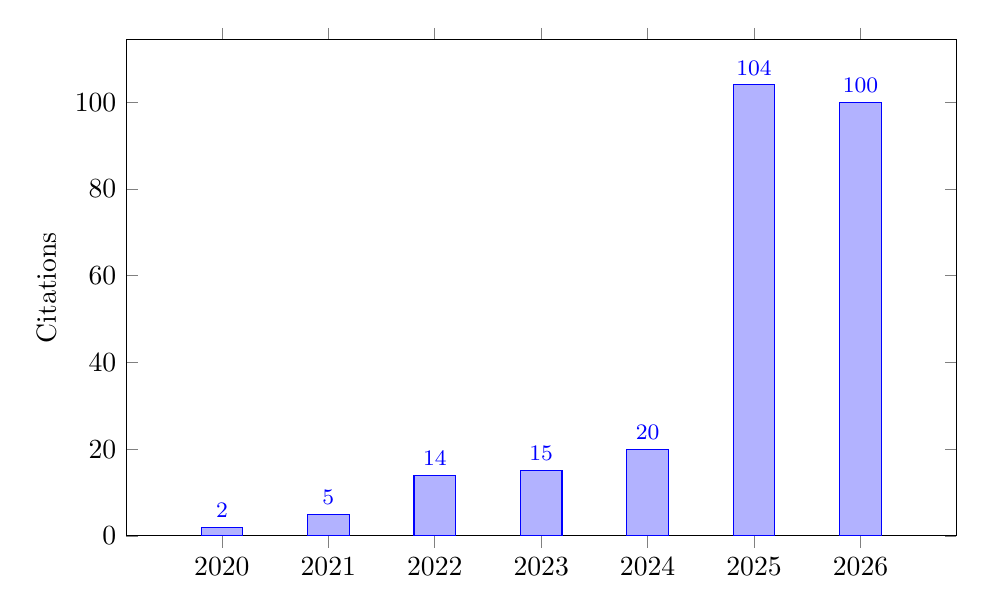
\begin{tikzpicture}
    \begin{axis}[
        ybar,
        bar width=15pt,
        ymin=0,
        ylabel={Citations},
        xtick=data,
        enlarge x limits=0.15,
        nodes near coords,
        every node near coord/.append style={font=\footnotesize},
        width=\linewidth,
        height=0.65\linewidth,
% AUTOGEN:CHART:START
        symbolic x coords={2020,2021,2022,2023,2024,2025,2026},
    ]
    \addplot coordinates {(2020,2) (2021,5) (2022,14) (2023,15) (2024,20) (2025,104) (2026, 100)};
% AUTOGEN:CHART:END
    \end{axis}
    \end{tikzpicture}
\end{minipage}
\hfill
% --- Right: Metrics Table in a minipage ---
\begin{minipage}[t]{0.4\textwidth}
    \vspace{-100pt}
    \begin{tabular}{@{}ll@{}}
% AUTOGEN:METRICS:START
        \textbf{\bodyfontlight Total Publications:}       &  16  \\
        \textbf{\bodyfontlight Total citations:} & 178 \\
        \textbf{\bodyfontlight h-index:}         & 6  \\
% AUTOGEN:METRICS:END
    \end{tabular}
\end{minipage}
\end{center}



\begin{enumerate}
\label{sec:llmpsych}

  \item \cvpub{\textbf{\bodyfontlight Large Language Models Display Human-like Social Desirability Biases in Big Five Personality Surveys\\} \textbf{\bodyfontlight{Aadesh Salecha}}, Molly E. Ireland, Shashanka Subrahmanya, João Sedoc, Lyle H. Ungar, and Johannes C. Eichstaedt. \emph{PNAS Nexus}, Vol. 3, No. 12, pg. e533, 2024. \href{https://doi.org/10.1093/pnasnexus/pgae533}{\textcolor{MidnightBlue}{academic.oup.com/pnasnexus/article/3/12/pgae533/7919163}}}
   \href{https://www.wired.com/story/chatbots-like-the-rest-of-us-just-want-to-be-loved/}{\textcolor{MidnightBlue}{WIRED Magazine Article: Chatbots, Like the Rest of Us, Just Want to Be Loved}}

\end{enumerate}

\cvsubsection{Journal Publications}
\begin{enumerate}
\setcounter{enumi}{1}

\label{sec:adampnas}
\item \cvpub{\textbf{\bodyfontlight Monitoring the Opioid Epidemic via Social Media Discussions.\\ } Adam Lavertu, Tymor Hamamsy, \textbf{\bodyfontlight{Aadesh Salecha}}, Delaney Smith, Johannes Eichstaedt, and Russ B Altman. \emph{Nature Partner Journals: Digital Medicine.} \href{https://www.nature.com/articles/s41746-025-01642-x}{\textcolor{MidnightBlue}{nature.com/articles/s41746-025-01642-x}}}

\label{sec:fakenewsjournal}
\item \cvpub{\textbf{\bodyfontlight Fake News Spreader Detection using Trust-based strategies in Social Networks with Bot Filtration.\\ } Bhavtosh Rath, \textbf{\bodyfontlight{Aadesh Salecha}}, and Jaideep Srivastava. \emph{Social Network Analysis and Mining (SNAM)} (2022)\\\href{https://doi.org/10.1007/s13278-022-00890-z}{\textcolor{MidnightBlue}{doi.org/10.1007/s13278-022-00890-z}}}

\item \cvpub{\textbf{\bodyfontlight Relationship between Citizen-Eyewitness Images and Audience Engagement with News.\\ } Jisu Kim, Jisu Huh, Bhavtosh Rath, \textbf{\bodyfontlight{Aadesh Salecha}}, and Jaideep Srivastava. \emph{Journalism Practice} (2021)\\ \href{https://doi.org/10.1080/17512786.2021.1882873}{\textcolor{MidnightBlue}{doi.org/10.1080/17512786.2021.1882873}}}

\label{sec:covidjournal}
\item \cvpub{\textbf{\bodyfontlight Influence of Emotions on Coping Behaviors in Crisis: A Computational Analysis of the COVID-19 Outbreak.\\ }
Hao Xu, Smitha Muthya Sudheendra, Jisu Huh, \textbf{\bodyfontlight{Aadesh Salecha}}, and Jaideep Srivastava.
\emph{Journal of Computational Social Science}, 7, 1599–1623 (2024).
\href{https://doi.org/10.1007/s42001-024-00282-7}{\textcolor{MidnightBlue}{https://doi.org/10.1007/s42001-024-00282-7}}}

\label{sec:oliversubmitted}
\item \cvpub{\textbf{\bodyfontlight The Language of Conflict Transformation - Assessing Psychological Change Patterns in Israeli-Palestinian Track Two Interactive Problem Solving.\\ } Oliver Fink, Wilfried Graf, Shashanka Subrahmanya, \textbf{\bodyfontlight{Aadesh Salecha}}, and Johannes Eichstaedt. \emph{Negotiation and Conflict Management Research} (2024)}

\label{sec:therapytrainer}
\item \cvpub{\textbf{\bodyfontlight TherapyTrainer: Using AI to Train Therapists in Written Exposure Therapy.\\ } Elizabeth C. Stade, Johannes C. Eichstaedt, Debra L. Kaysen, \textbf{\bodyfontlight{Aadesh Salecha}}, Alanna Greenberger, Shreya Singhvi, and Shannon Wiltsey Stirman. \emph{Cognitive and Behavioral Practice} (2025)}

\label{sec:crqpublished}
\item \cvpub{\textbf{\bodyfontlight No Good Time to Negotiate? Effective Track Two Dialogue in Protracted Israel-Palestine Conflict Escalation.\\ } Oliver Fink, Wilfried Graf, Shashanka Subrahmanya, \textbf{\bodyfontlight{Aadesh Salecha}}, and Johannes Eichstaedt. \emph{Conflict Resolution Quarterly} (2026)\\\href{https://doi.org/10.1002/crq.70032}{\textcolor{MidnightBlue}{doi.org/10.1002/crq.70032}}}

\end{enumerate}

\cvsubsection{Conference Publications}
\begin{enumerate}
\setcounter{enumi}{8}

\item \cvpub{\textbf{\bodyfontlight Emergence and Stability of Self-Evolved Cooperative Strategies using Stochastic Machines.\\ } Jin Hong Kuan, and \textbf{\bodyfontlight{Aadesh Salecha}}. In \emph{IEEE Symposium Series on Computational Intelligence (SSCI)} (2020) \\\href{https://ieeexplore.ieee.org/abstract/document/9308258}{\textcolor{MidnightBlue}{https://ieeexplore.ieee.org/abstract/document/9308258}}}

\label{sec:fakenewsconference}
\item \cvpub{\textbf{\bodyfontlight Detecting Fake News Spreaders in Social Networks using Inductive Representation Learning.\\ } Bhavtosh Rath, \textbf{\bodyfontlight{Aadesh Salecha}}, and Jaideep Srivastava. In \emph{IEEE/ACM International Conference on Advances in Social Networks Analysis and Mining (ASONAM)} (2020) \href{https://ieeexplore.ieee.org/abstract/document/9381466}{\textcolor{MidnightBlue}{https://ieeexplore.ieee.org/abstract/document/9381466}}}

\label{sec:icaconference}
\item \cvpub{\textbf{\bodyfontlight Public's Discrete Emotions During the COVID-19 and Impacts on Their Coping Behaviors in the U.S.\\ } Hao Xu, Smitha Muthya Sudheendra, Jisu Huh, \textbf{\bodyfontlight{Aadesh Salecha}}, and Jaideep Srivastava. \emph{72nd Annual International Communication Association Conference} (2022)}

\end{enumerate}

\cvsubsection{Under Review}

\begin{enumerate}[]
\setcounter{enumi}{11}

\item \cvpub{\textbf{\bodyfontlight A Computational Model of Reward Learning and Habits on Social Media\\ } Georgia Turner, Lukas J. Gunschera, Shashanka Subrahmanya, \textbf{\bodyfontlight{Aadesh Salecha}}, Johannes C. Eichstaedt, Stefano Palminteri, and Amy Orben. Accepted, \emph{Nature Communications}. \href{https://osf.io/preprints/psyarxiv/xe25k}{\textcolor{MidnightBlue}{osf.io/preprints/psyarxiv/xe25k}}}

\item \cvpub{\textbf{\bodyfontlight The answer to the mental health crisis: Examining media bias regarding psychedelic treatments for depression and PTSD using natural language processing.\\} {{Audrey Evers, Elizabeth C. Stade, \textbf{\bodyfontlight Aadesh Salecha}, Zoe Tait, Gabriela Khazanov.}}}

% \label{sec:oliverstrategic}
% \item \cvpub{\textbf{\bodyfontlight No Good Time to Negotiate? Track Two Diplomacy within the Protracted Israel-Palestine Conflict as Strategic Joint Thinking.\\ } Oliver Fink, Wilfried Graf, Shashanka Subrahmanya, \textbf{\bodyfontlight{Aadesh Salecha}}, and Johannes Eichstaedt. To be submitted to \emph{Journal of Conflict Resolution} (revisions pending)}

\label{sec:wellbeing}
\item \cvpub{\textbf{\bodyfontlight Structured AI Dialogues Can Increase Happiness and Meaning in Life\\ } \textbf{\bodyfontlight Aadesh Salecha}, Jonas Schöne, Sonja Lyubomirsky, João Sedoc, Johannes Eichstaedt, and Robb Willer.}

\label{sec:likescovid}
\item \cvpub{\textbf{\bodyfontlight Increased Behavioural Sensitivity to `Likes' During the COVID-19 Pandemic.\\ } Brandon C. Davidson, \textbf{\bodyfontlight{Aadesh Salecha}}, et al. Submitted to \emph{Psychological Science} (2026)}

\end{enumerate}

\cvsubsection{Theses}

\begin{enumerate}[]
\setcounter{enumi}{15}
\item \cvpub{\textbf{\bodyfontlight Empirical Study of the Spread of Misinformation: A Big Data Approach.\\ } \textbf{\bodyfontlight{Aadesh Salecha}}. Undergraduate Thesis (Summa Cum Laude). Retrieved from the \emph{University of Minnesota Digital Conservancy} (2021). \href{https://hdl.handle.net/11299/222250}{\textcolor{MidnightBlue}{{https://hdl.handle.net/11299/222250}}}}
\end{enumerate}

% AUTOGEN:NEWPUBS:START
% New Google Scholar publications not matched (by title) to anything else in this file
% are listed here automatically. Move each into the right section above with its own
% \label and citation style, then delete it from this block.
% AUTOGEN:NEWPUBS:END

% \cvsubsection{Preprints}

% \begin{enumerate}
% \setcounter{enumi}{13}
% \item \cvpub{\textbf{\bodyfontlight Time Complexity Analysis of an Evolutionary Algorithm for approximating Nash Equilibriums.\\ } \textbf{\bodyfontlight{Aadesh Salecha}}. arXiv preprint arXiv:2110.13563 (2021). \href{https://arxiv.org/abs/2110.13563}{\textcolor{MidnightBlue}{https://arxiv.org/abs/2110.13563}}}
% \end{enumerate}
%-------------------------------------------------------------------------------
% SECTION TITLE
%-------------------------------------------------------------------------------

\cvsection{Press Coverage}

\begin{enumerate}
  \item \cvpub{\textbf{\bodyfontlight Chatbots, Like the Rest of Us, Just Want to Be Loved.\\ } \textbf{\bodyfontlight Wired}}. Published on March 5, 2025. Retrieved from \href{https://www.wired.com/story/chatbots-like-the-rest-of-us-just-want-to-be-loved/}{\textcolor{MidnightBlue}{https://www.wired.com/story/chatbots-like-the-rest-of-us-just-want-to-be-loved/}}
  
  \item \cvpub{\textbf{\bodyfontlight Breaking Negative Thought Patterns Could Ward Off Anxiety, Depression.\\ } \textbf{\bodyfontlight Science News}}. Published in February 2025. Retrieved from \href{https://www.sciencenews.org/article/negative-thoughts-anxiety-depression}{\textcolor{MidnightBlue}{https://www.sciencenews.org/article/negative-thoughts-anxiety-depression}}
  
  \item \cvpub{\textbf{\bodyfontlight Are AI Chatbot 'Personalities' in the Eye of the Beholder?\\ } \textbf{\bodyfontlight Science News}}. Published in February 2025. Retrieved from \href{https://www.sciencenews.org/article/ai-chatbot-personalities}{\textcolor{MidnightBlue}{https://www.sciencenews.org/article/ai-chatbot-personalities}}
  
  \item \cvpub{\textbf{\bodyfontlight Large Language Models Just Want to Be Liked.\\ } \textbf{\bodyfontlight Stanford HAI}}. Published on January 13, 2025. Retrieved from \href{https://hai.stanford.edu/news/large-language-models-just-want-be-liked}{\textcolor{MidnightBlue}{https://hai.stanford.edu/news/large-language-models-just-want-be-liked}}

  % MIT High School Student interview https://storymaps.arcgis.com/collections/b31a4f9c586b4c688ae6fbad36284631?item=10
\end{enumerate}

% \vspace{-8mm}
%-------------------------------------------------------------------------------
%	SECTION TITLE
%-------------------------------------------------------------------------------
\cvsection{Academic Work Experience}

\vspace{-3mm}
\begin{cvskills}

\cventry{AI/ML Scientist}{\href{https://cpwb.stanford.edu/people}{Computational Psychology \& Well-Being Lab}}{Stanford University}{May 2023 -- Present} 
{
\begin{cvitems}
\item[] Technologies: \emph{Differential Language Analysis, Large Language Models}
\item[] Mentored by \textit{\href{https://hai.stanford.edu/people/johannes-eichstaedt}{Prof. Johannes Eichstaedt}}
\item Developing  \textbf{\bodyfontlight LLM evaluation metrics} to measure \textbf{\bodyfontlight behavioral} strengths and \textbf{\bodyfontlight biases} based on psychological principles\textbf{\bodyfontlight \hyperref[sec:llmpsych]{\textsuperscript{[8]}}}
\item Creating \textbf{\bodyfontlight AI-assisted} variants of well-established and novel positive-psychology \textbf{\bodyfontlight interventions} to improve well-being\textbf{\bodyfontlight \hyperref[sec:wellbeing]{\textsuperscript{[11]}}}
% Developing applications using LLMs for mental health screening and well-being intervention delivery
% \item Applying advanced NLP techniques to extract, and analyze large-scale language data from social media platforms
\item Applying advanced \textbf{\bodyfontlight NLP} techniques to novel domains like \textbf{\bodyfontlight conflict mediation} talks between \textbf{\bodyfontlight Israel \& Palestine}\textbf{\bodyfontlight \hyperref[sec:oliversubmitted]{\textsuperscript{[9,}}}\textbf{\bodyfontlight \hyperref[sec:oliverprep]{\textsuperscript{10]}}}
\item Facilitating measurement and causal analysis of \textbf{\bodyfontlight population health metrics like opioid usage}\textbf{\bodyfontlight \hyperref[sec:adampnas]{\textsuperscript{[4]}}} and subjective well-being
\end{cvitems}
}
\end{cvskills}

\vspace{-1.5mm}
\begin{cvskills}
\cventry{Research Assistant}{Data Analysis and Management Research Group}{University of Minnesota}{Feb 2019 -- Dec 2022} 
{
\begin{cvitems}
\item[] Technologies: \emph{Graph Neural Networks, NoSQL}
\item[] Mentored by \textit{\href{https://cse.umn.edu/cs/jaideep-srivastava}{Prof. Jaideep Srivastava}}
\item Curated a dataset of 10 unique news events and 50 million associated users and their follower-followee networks\textbf{\bodyfontlight \hyperref[sec:fakenewsconference]{\textsuperscript{[6]}}}
\item Published methods that leverage inter-user trust to {\textbf{\bodyfontlight detect fake news spreaders}} with an accuracy of 93\%\textbf{\bodyfontlight \hyperref[sec:fakenewsjournal]{\textsuperscript{[1]}}}
% \item Demonstrated performance benefits (3\% increase in accuracy) arising from bot-filtration
% \item Studying public emotions towards COVID and its effects on social-distancing compliance
\item Analyzed people's information seeking/sharing behavior in relation to COVID-19 social-distancing compliance\textbf{\bodyfontlight \hyperref[sec:covidjournal]{\textsuperscript{[3,}}}\textbf{\bodyfontlight \hyperref[sec:icaconferencef]{\textsuperscript{7]}}}
\end{cvitems}
}
\end{cvskills}

% \\ 

% \vspace{-2mm}
% \cventry{Undergraduate Research Assistant}{Computation, Motivation, and Control Laboratory}{University of Minnesota}{Feb 2019 -- Mar 2020} 
% {
% % Technologies: Pytorch, Word2Vec, Keras
% \begin{cvitems}
% \item[] Technologies: \emph{Contextual Word Embeddings, Knowledge Graphs, Time Series}
% \item[] Mentored by \textit{\href{https://cse.umn.edu/cs/paul-schrater}{Prof. Paul Schrater}}
% \item Leveraged deep-learning visual models and knowledge graphs to construct novel feature sets for eye-tracking data
% \item Designed state-of-the-art saliency detection and \textbf{\bodyfontlight eye-scanpath prediction models}
% \item Created novel Transformer architectures for \textbf{\bodyfontlight mental health diagnosis using viewing behavior}
% \end{cvitems}
% }

% \end{cvskills}

% \pagebreak

\vspace{-2mm}
\cvsection{Industry Experience}

\begin{cvskills}

\cventry{AI/ML Software Engineer}{\href{https://aws.amazon.com/sagemaker-ai/hyperpod/}{Amazon (AWS)}}{Seattle}{June 2025 -- Sept 2025} 
{
\begin{cvitems}
\item[] Technologies: \emph{Large Language Models, RAG, Agentic AI, Prometheus, Grafana, CloudWatch} 
\item Designed an \textbf{\bodyfontlight agentic AI system} leveraging \textbf{\bodyfontlight RAG} to autonomously diagnose and resolve ML training failures across distributed GPU clusters
    \item Integrated telemetry data (Prometheus, Grafana, CloudWatch) into a data–model feedback loop for \textbf{\bodyfontlight predictive maintenance} and system reliability
    \item Improved compute efficiency and reduced manual effort, cutting operational costs and lowering \textbf{\bodyfontlight carbon emissions by 200 kg CO$_2$e per day}
\end{cvitems}
}

\\

% \vspace{-11mm}
\cventry{Senior Software Engineer}{DraftKings Inc.}{Boston}{Dec 2021 -- Jun 2024} 
{
\begin{cvitems}
\item[] Technologies: \emph{.NET, MySQL, AWS, RabbitMQ, Octopus Deploy}
\item Co-developed a \textbf{\bodyfontlight distributed accounting ledger system} to store millions of user transactions
\item Delivered \textbf{\bodyfontlight full-stack} solutions, micro-services to handle billions of requests with <200ms latencies
\item \textbf{\bodyfontlight Led cross-functional} initiatives to elevate user experience and reduce dropout by 40\%
% \item Working with project managers and team members to maintain and scale services using AWS resources
\end{cvitems}
}

\\

\cventry{Data Scientist}{Blue Zones, LLC}{Remote}{Jun 2023 - Jan 2024} 
{
\begin{cvitems}
\item[] Worked with \textit{\href{https://www.bluezones.com/dan-buettner/}{Dan Buettner}}, New York Times best-selling author
\item Curated a novel \textbf{\bodyfontlight dataset of over 1 million recipes}, analyzing American culinary preferences
\item Leveraged advanced \emph{data mining techniques} to pinpoint recipe candidates for Dan Buettner's upcoming book
\item Implemented a \textbf{\bodyfontlight production-grade} recipe generation bot using \textbf{\bodyfontlight RAG, and advanced prompt engineering} techniques
\end{cvitems}
}
% \cventry{Teaching Assistant}{Department of Computer Science}{University of Minnesota}{Jan 2020 -- May 2021} 
% {
% \begin{cvitems}
% \item Taught \textbf{\bodyfontlight discussion sections for 40+ students} using self-curated lesson plans, and problem sheets
% \item Facilitated grading and proctoring for over 80 projects and exams over \textbf{\bodyfontlight 4 semesters}
% \item Instructed students individually and in groups through office-hours
% \end{cvitems}
% } 

% \cventry{Peer Learning Tutor}{SMART Learning Commons}{University of Minnesota}{Feb 2020 -- May 2021} 
% {
% \begin{cvitems}
% \item Consistently ranked in the top 5 most visited tutors amongst a group of 50+ tutors
% \item Tutored for 40+ courses ranging from Calculus 1 to Artificial Intelligence II
% \item Mentored 10 fellow tutors on effective strategies for addressing student needs
% \end{cvitems}
% }

% \\ 

% \cventry{Hospitality Specialist}{Housing and Residential Life}{University of Minnesota}{Nov 2018 -- Nov 2020} 
% {
%  \begin{cvitems}
% \item Served as a Community Advisor to a group of 50 students and built a safe environment for residents
% \item Supervised administrative tasks of day-to-day business operations
% \item Assisted with building maintenance and custodial duties
% \end{cvitems}
% }

% \\ 

% \cventry{Software Engineering Intern}{HION Events Pvt Ltd}{Bangalore, India}{Feb 2018 -- July 2018} 
% {
%  \begin{cvitems}
% \item[] Technologies: \emph{Matlab, Cypress toolkit, Embedded C}
% \item Conceptualized and prototyped an IoT wearable smartwatch from scratch in the span of 6 months
% \item Developed ML models that could recognize 20+ unique gestures
% \item Wrote efficient code to run in real-time on embedded systems
% \end{cvitems}
% }

\end{cvskills}

% \cventry{Peer Learning Tutor}{SMART Learning Commons}{University of Minnesota}{Feb 2020 -- May 2021} 
% {
% \begin{cvitems}
% \item Consistently ranked in the top 5 most visited tutors amongst a group of 50+ tutors
% \item Tutored for 40+ courses ranging from Calculus 1 to Artificial Intelligence II
% \item Mentored 10 fellow tutors on effective strategies for addressing student needs
% \end{cvitems}
% }

% \\ 

% \cventry{Hospitality Specialist}{Housing and Residential Life}{University of Minnesota}{Nov 2018 -- Nov 2020} 
% {
%  \begin{cvitems}
% \item Served as a Community Advisor to a group of 50 students and built a safe environment for residents
% \item Supervised administrative tasks of day-to-day business operations
% \item Assisted with building maintenance and custodial duties
% \end{cvitems}
% }


% \\ 

% \cventry{Software Engineering Intern}{HION Events Pvt Ltd}{Bangalore, India}{Feb 2018 -- July 2018} 
% {
%  \begin{cvitems}
% \item[] Technologies: \emph{Matlab, Cypress toolkit, Embedded C}
% \item Conceptualized and prototyped an IoT wearable smartwatch from scratch in the span of 6 months
% \item Developed ML models that could recognize 20+ unique gestures
% \item Wrote efficient code to run in real-time on embedded systems
% \end{cvitems}
% }

% \divider

% \cvevent{Teaching Assistant}{Department of Computer Science, University of Minnesota}{Jan 2020 -- May 2021}{}
% Courses: \emph{Intro to DS \& Algo}, \emph{Discrete Mathematics} \emph{Computational Linear Algebra}, and \emph{Advanced Programming Principles}
% \begin{itemize}
% \item Led and taught a discussion section for a group of 43 students
% \item Facilitated grading and proctoring for over 80 projects and exams over 4 semesters
% \item Instructed students individually and in groups to learn complex computer science concepts during office-hours
% \end{itemize}

% \divider

% \cvevent{Peer Learning Tutor}{SmartLearning Commons}{Feb 2020 -- May 2021}{}
% \begin{itemize}
% \item Consistently ranked in the top 5 most visited tutors 
% \item Tutored for courses ranging from Calculus 1 to Artificial Intelligence 2
% \item Mentored 10 fellow tutors on how to address student needs specifically for Computer Science subjects
% \end{itemize}

% \divider

% \cvevent{Software Engineering Intern}{HION Events Pvt Ltd, India}{Feb 2018 - Juy 2018}{}
%  Technologies: Matlab, Cypress toolkit, Embedded C
%  \begin{itemize}
% \item Conceptualized and prototyped an IoT wearable smartwatch from scratch in the span of 6 months
% \item Developed ML models that could recognize 20+ unique gestures
% \item Wrote efficient code to run in real-time on embedded systems
% \end{itemize}
% \divider

% \pagebreak
%-------------------------------------------------------------------------------
%	SECTION TITLE
%-------------------------------------------------------------------------------
\newpage
\cvsection{Awards \& Honors}

\begin{cvhonors}

%---------------------------------------------------------
  \cvhonor
    {\textbf{Undergraduate Research Opportunity Grant}} % Award
    {Office of Research Opportunities} % Awarding Organization
    {\textbf{\$3000.00}} % Amount
    {2020} % Date(s)

%---------------------------------------------------------
  \cvhonor
    {\textbf{Tom Niccum Travel Grant}} % Award
    {College of Science and Engineering} % Awarding Organization
    {\textbf{\$1000.00}} % Amount
    {} % Date(s)

\end{cvhonors}


\begin{cvhonors}
%---------------------------------------------------------
  \cvhonor
    {\textbf{Google’s CS Research Mentorship Program Nominee}} % Award
    {Google, Inc.} % Awarding Organization
    {} % Amount
    {2019} % Date(s)
    
%---------------------------------------------------------
  \cvhonor
    {\textbf{Dean’s List - Spring 2019}} % Award
    {College of Science and Engineering} % Awarding Organization
    {} % Amount
    {} % Date(s)

%---------------------------------------------------------
  \cvhonor
    {\textbf{Dean’s List - Fall 2019}} % Award
    {College of Science and Engineering} % Awarding Organization
    {} % Amount
    {} % Date(s)

\end{cvhonors}


%-------------------------------------------------------------------------------
%	2018
%-------------------------------------------------------------------------------
\begin{cvhonors}

%---------------------------------------------------------
  \cvhonor
    {\textbf{ExxonMobil Scholarship }} % Award
    {ExxonMobil via Computer Science Department, UMN} % Awarding Organization
    {\textbf{\$3000.00}} % Amount -- leave blank if not including amounts
    {2018} % Date(s)

%---------------------------------------------------------
  \cvhonor
    {\textbf{Dean’s List - Fall 2018}} % Award
    {College of Science and Engineering} % Awarding Organization
    {} % Amount
    {} % Date(s)

\end{cvhonors}


%-------------------------------------------------------------------------------
%	SECTION TITLE
%-------------------------------------------------------------------------------
\cvsection{Conference Presentations}

% \cvsubsection{Oral Presentations}
%-------------------------------------------------------------------------------

\begin{cvpubs}

\cvpub{\quad \quad Kuan, Jin Hong, and \textbf{\bodyfontlight{Aadesh Salecha}}. "Emergence and Stability of Self-Evolved Cooperative Strategies using Stochastic Machines.'' \emph{IEEE Symposium Series on Computational Intelligence (SSCI)}, Canberra, Australia. (2020)} % (held virtually due to the pandemic)

% \item \cvpub{\textbf{\bodyfontlight{Aadesh Salecha}}. ``Time Complexity Analysis of an Evolutionary Algorithm for approximating Nash Equilibriums.'' arXiv preprint arXiv:2110.13563 (2021). \href{https://arxiv.org/abs/2110.13563}{\textcolor{MidnightBlue}{https://arxiv.org/abs/2110.13563}}}
% \end{enumerate}


    % \cvpub{Undergrad, Y*\textsuperscript{+}, \textbf{Your Name}, Author Three, Author Four. 2015. Title of a poster presented by an undergrad I mentored. Poster: Event Presented At, City, State.}
% \end{enumerate}
    
\end{cvpubs}

%-------------------------------------------------------------------------------
% SECTION TITLE
%-------------------------------------------------------------------------------
\cvsection{Teaching Experience}

% \begin{cvparagraph}
    
% \end{cvparagraph}

\begin{cvpubs}
    \cvpub{\quad \quad \quad \quad \quad \quad \quad \textbf{\bodyfontlight{Average Student Rating: 4.75/5, \quad Total Teaching Hours: 900+ hours}}}
    % \cvpub{\quad \quad \quad \quad \quad \quad \textbf{\bodyfontlight{CRLA International Tutor Training Program Certified (Level 1)}}}
\end{cvpubs}

% As a Teaching Assistant:
\begin{cvhonors}
\cvhonor
{\bodyfont{OIT 274: {Data and Decisions}}}
{Teaching Assistant with Prof. \href{https://www.gsb.stanford.edu/faculty-research/faculty/claudia-allende-santa-cruz}{Claudia Santa Cruz}}
{}
{Winter '25}
\end{cvhonors}

\begin{cvhonors}
\cvhonor
{\bodyfont{OIT 247: {Optimization and Simulation Modeling - Accelerated}}}
{Teaching Assistant with \href{https://stanford.edu/~kostasb/}{Prof. Kostas Bimpikis}}
{}
{Autumn '25}
\end{cvhonors}

\begin{cvhonors}
\cvhonor
{\bodyfont{CSCI 2033: {Computational Linear Algebra}}}
{Teaching Assistant with Prof. Carl Sturtivant}
{}
{Spring '21}
\end{cvhonors}


\begin{cvhonors}

\cvhonor
{\bodyfont{CSCI 1933: {Intro to DS \& Algo}}}
{Teaching Assistant with Prof. James Polzin}
{}
{Summer '20}
\end{cvhonors}


\begin{cvhonors}
\cvhonor
{\bodyfont{CSCI 2041: {Advanced Programming Principles}}}
{Teaching Assistant with Prof. Eric Van Wyk}
{}
{Fall '20}
\end{cvhonors}
% \begin{itemize} 
% \item Led and taught a discussion section for a group of 43 students using self-curated lesson plans, slide decks and problem sheets.
% % \item Graded midterms, weekly quizzes and final exam. \item Held weekly office hours.
% \end{itemize}

% }


\begin{cvhonors}
\cvhonor
{\bodyfont{CSCI 2011: {Discrete Mathematics}}}
{Teaching Assistant with Prof. Kate Jensen}
{}
{Spring '20}
\end{cvhonors}
% {\cvparagraph


% \textbf{As a Peer Tutor:}
\begin{cvhonors}
\cvhonor
{\bodyfont{Computer Science, Mathematics, and Physics}}
{Peer Tutor at SMART Learning Commons}
{}
{Spring '20 -- '21}
\end{cvhonors}
\hfill\begin{minipage}{\textwidth-2.1cm}
\doublespacing
{\cvparagraph
% Courses supported over 4 semesters (425+ hours of tutoring)
% \begin{itemize} 
% \item CSCI 1133 / CSCI 1113: Introduction to Computer Science with Python / C++
% \item CSCI 2011: Discrete Structures of Computer Science
% \item CSCI 2021: Machine Architecture and Organization
% \item CSCI 2033: Elementary Computational Linear Algebra
% \item CSCI 2041: Advanced Programming Principles
% \item CSCI 4041: Algorithms and Data Structures
% \item CSCI 4511W: Introduction to Artificial Intelligence
% \item CSCI 4061: Introduction to Operating Systems
% \item CSCI 5512: Artificial Intelligence II
% \item CSCI 5521: Machine Learning Fundamentals
% \item MATH 4707: Intro to Combinatorics and Graph Theory
% \item MATH 5165: Math Logic I
% \item PSY 5018H: Math Models of Human Behavior
% \end{itemize}

}
\end{minipage}

% \cvhonor
% {CSCI 2041: {Advanced Programming Principles}}
% {Peer Tutor}
% {}
% {Spring 2020}

% \cvhonor
% {CSCI 2041: {Advanced Programming Principles}}
% {Peer Tutor}
% {}
% {Spring 2020}

% \cvhonor
% {CSCI 2041: {Advanced Programming Principles}}
% {Peer Tutor}
% {}
% {Spring 2020}



% %---------------------------------------------------------

%-------------------------------------------------------------------------------
%	SECTION TITLE
%-------------------------------------------------------------------------------
\cvsection{Academic  Service}


%-------------------------------------------------------------------------------
%	CONTENT
%-------------------------------------------------------------------------------
%---------------------------------------------------------

\begin{cvhonors}    
\cvhonor
    {\textbf{Committee Member}} % Relationship
    {16th International Conference on Advanced Engineering Computing and Applications in Sciences (ADVCOMP)} % Name
    {} % Location
    {2022} % Date(s)
\end{cvhonors}

\begin{cvhonors}

\cvhonor
    {\textbf{Peer Reviewer}} % Relationship
    {Minnesota Undergraduate Research \& Academic Journal (MURAJ)} % Name
    {} % Location
    {2020 - 2021} % Date(s)
    
\end{cvhonors}

\begin{cvpubs}
    \cvpub{
    \quad \quad \quad \quad \quad \quad \quad \href{https://pubs.lib.umn.edu/index.php/muraj/article/view/4019/2767}{\-\ Peer Reviewed 2 articles published in Volume 4, Issue 5 of the MURAJ Undergraduate Journal}
    % \newline  
    % \-\ \-\ \-\ \-\ \-\ \-\ \-\ \-\ \-\ \-\ \-\ \-\ \-\ \-\ \-\ \-\ \-\ \-\ \-\ \-\ \-\ \-\ \-\ \-\ \-\  \href{}{Link to proceedings: https://pubs.lib.umn.edu/index.php/muraj/article/view/4019/2767}
    }
\end{cvpubs}

%-------------------------------------------------------------------------------
\end{document}
